% =============================================================================
% Relatório do projeto CineGraph — PTC3567 Ciência dos Dados (Poli-USP)
%
% Compilar:  tectonic relatorio.tex   (ou latexmk -pdf relatorio.tex, ou Overleaf
% com a pasta relatorio/ inteira). As figuras vêm de figuras/gerar_figuras.py.
% =============================================================================
\documentclass[11pt,a4paper]{article}

\usepackage{iftex}
\ifPDFTeX
  \usepackage[utf8]{inputenc}
  \usepackage[T1]{fontenc}
  \usepackage{lmodern}
\else
  \usepackage{fontspec}
\fi
\usepackage[brazil]{babel}
\usepackage{icomma}
\usepackage[margin=2.5cm]{geometry}
\usepackage{microtype}
\setlength{\emergencystretch}{3em}
\setlength{\parskip}{0.35em}
\usepackage{amsmath}
\usepackage{graphicx}
\usepackage{booktabs}
\usepackage{tabularx}
\usepackage{array}
\usepackage{xcolor}
\usepackage{caption}
\captionsetup{font=small,labelfont=bf,skip=5pt}
\usepackage{enumitem}
\setlist{itemsep=1pt,topsep=3pt}
\usepackage{fancyvrb}
\usepackage{tikz}
\usetikzlibrary{arrows.meta}
\usepackage{csquotes}
\usepackage[hidelinks,unicode]{hyperref}
\usepackage{url}
\usepackage[alf]{abntex2cite}

\definecolor{azul}{HTML}{2A78D6}
\definecolor{laranja}{HTML}{E08A1E}
\definecolor{tinta}{HTML}{1A1A19}
\definecolor{cinza}{HTML}{52514E}
\definecolor{fundo}{HTML}{F4F2EC}
\definecolor{fundoazul}{HTML}{DCE6F7}
\definecolor{fundolaranja}{HTML}{F7E6CC}

\newcommand{\cg}{CineGraph}
\newcommand{\code}[1]{\texttt{#1}}
% Caminhos em fonte mono, sem os sinais < > que o abntex2cite põe nos URLs.
\DeclareUrlCommand\arq{\urlstyle{tt}\def\UrlLeft{}\def\UrlRight{}}
% Endereço do repositório de código.
\newcommand{\urlrepositorio}{\href{https://github.com/vinikenji10/cinegraph}{\arq{https://github.com/vinikenji10/cinegraph}}}
\fvset{fontsize=\small,frame=single,framesep=5pt,rulecolor=\color{cinza!60}}

\hypersetup{pdftitle={CineGraph: chatbot híbrido para recomendação de filmes},
  pdfauthor={Gustavo Jae Min Yu, Ian Seo Takose, Vinicius Kenji Yamada}}

\begin{document}

% =============================================================================
% CAPA
% =============================================================================
\begin{titlepage}
  \centering
  
\includegraphics[width=3.4cm]{figuras/logo-poli.jpg}\par
  \vspace{0.7cm}
  {\large\textbf{UNIVERSIDADE DE SÃO PAULO}}\par
  \vspace{2pt}
  {\large\textbf{ESCOLA POLITÉCNICA}}\par
  \vspace{6pt}
  PTC3567 -- Ciência dos Dados\par
  \vfill
  {\Huge\bfseries CineGraph}\par
  \vspace{0.4cm}
  {\Large Chatbot híbrido para recomendação de filmes}\par
  \vspace{0.6cm}
  {\large Relatório do projeto da disciplina}\par
  \vfill
  \begin{tabular}{l@{\hspace{1.5cm}}r}
    \toprule
    \textbf{Integrante} & \textbf{N\textsuperscript{o} USP} \\
    \midrule
    Gustavo Jae Min Yu    & 13782762 \\
    Ian Seo Takose        & 13680592 \\
    Vinicius Kenji Yamada & 13782863 \\
    \bottomrule
  \end{tabular}\par
  % \vspace{0.5cm} Professores: Prof.\ Dr.\ NOME e Prof.\ Dr.\ NOME\par
  \vfill
  São Paulo, novembro de 2026\par
\end{titlepage}

% =============================================================================
\section{Introdução}
% =============================================================================

\subsection{Problema}

Pedidos de recomendação de filmes misturam critérios objetivos, como gênero, ano e nota
(\enquote{os 5 filmes de ação mais bem avaliados depois de 2015}), e subjetivos, como tema,
atmosfera ou semelhança (\enquote{algo melancólico sobre memória e identidade}). Consultas
SQL respondem com exatidão aos primeiros, mas não têm como representar
\enquote{melancólico}. Um modelo de linguagem (LLM) entende os dois tipos, mas responde de
memória e pode inventar títulos, anos, gêneros ou notas \cite{ji2023hallucination}.

O projeto investigou \textbf{como combinar consultas estruturadas e busca semântica para
gerar recomendações relevantes e verificáveis}. Construímos o \cg, um chatbot em que um
grafo LangGraph classifica cada pergunta e escolhe entre \emph{Text-to-SQL}, busca vetorial
e um modo híbrido. Testamos quatro hipóteses: \textbf{H1}, o SQL é mais preciso em perguntas
objetivas; \textbf{H2}, a busca vetorial é mais relevante em perguntas semânticas;
\textbf{H3}, o modo híbrido é melhor em perguntas mistas; \textbf{H4}, o sistema roteado
inventa menos dados que um chatbot só com o LLM.

\subsection{Experimentos semelhantes}

O \cg\ segue a ideia de geração aumentada por recuperação (RAG), em que o modelo responde
condicionado a documentos recuperados \cite{lewis2020rag}. Dois trabalhos recentes tratam
problemas próximos:

\begin{itemize}
  \item \textbf{InteRecAgent} \cite{huang2025interecagent}: um LLM (GPT-4) coordena
        ferramentas de recomendação. Condições rígidas do pedido (atributos explícitos) são
        resolvidas por SQL, e condições flexíveis (semelhança) por ferramentas item a item;
        os candidatos circulam fora do \emph{prompt}. Avaliado com usuário simulado nas
        bases Steam, MovieLens e Amazon Beauty, superou LLMs de uso geral. O \cg\ adota a
        mesma divisão entre condições rígidas e flexíveis, usando busca semântica no lugar
        da ferramenta colaborativa, e mede explicitamente os dados inventados.
  \item \textbf{TAG} \cite{biswal2025tag}: mostra que \emph{Text-to-SQL} e RAG, isolados,
        atendem só parte das perguntas sobre bancos de dados (os métodos padrão acertam no
        máximo 20\% do \emph{benchmark} dos autores) e propõe três etapas: síntese da
        consulta, execução e geração. O modo híbrido do \cg\ é uma instância simples disso:
        similaridade vetorial para a parte subjetiva, filtro relacional exato para a
        objetiva e geração só sobre o resultado.
\end{itemize}

% =============================================================================
\section{Estratégias de Gestão dos Dados}
% =============================================================================

\textbf{Fontes.} Os dados são o MovieLens Latest Small, do GroupLens Research
(Universidade de Minnesota), obtido em
\arq{https://files.grouplens.org/datasets/movielens/ml-latest-small.zip}. A citação exigida
pela licença é \citeonline{harper2015movielens}, DOI
\href{https://doi.org/10.1145/2827872}{\arq{10.1145/2827872}}. Os vetores usam o modelo
\code{paraphrase-multilingual-\allowbreak MiniLM-L12-v2} \cite{reimers2020multilingual}, DOI
\href{https://doi.org/10.18653/v1/2020.emnlp-main.365}{\arq{10.18653/v1/2020.emnlp-main.365}},
executado localmente; o LLM é o Claude Sonnet 5.5 (\code{claude-sonnet-5-5}), via API.

\textbf{Plano de gestão de dados.} O plano, mantido em \arq{docs/DMP.md}, define:
\begin{itemize}
  \item \emph{Licença}: o MovieLens não pode ser redistribuído, então os dados ficam fora do
        repositório e cada integrante os recria por \emph{script}.
  \item \emph{Versão congelada}: o conjunto \enquote{Latest} muda com o tempo; o comando
        \code{cinegraph download} confere o MD5 publicado
        (\code{31a303aabbc519bd33d025e44d6c2570}) e grava um manifesto com o SHA-256 de
        cada CSV. Execuções seguintes falham se o conteúdo mudar.
  \item \emph{Acesso}: segredos fora do Git; banco SQLite aberto só para leitura; Firestore
        acessível apenas pelo \emph{backend}; site restrito a contas \code{@usp.br}.
  \item \emph{Privacidade}: o MovieLens usa identificadores anônimos; o site guarda o
        histórico apenas pelo \code{uid} do usuário.
\end{itemize}

\textbf{Reprodutibilidade.} As versões das bibliotecas estão travadas em \code{uv.lock}; o
modelo, as versões dos \emph{prompts} e os parâmetros ficam registrados no código e em cada
execução da avaliação, que grava também todas as respostas brutas. O \emph{bootstrap} usa
semente 42. Como o LLM é um serviço externo e pode variar, os resultados deste relatório se
referem a uma execução identificada (\code{20261117-173343}, custo de US\$ 4,33). Tudo se
reproduz com:

\begin{Verbatim}
uv sync && uv run cinegraph download && uv run cinegraph build-db
uv run cinegraph build-index && uv run cinegraph eval
\end{Verbatim}

\textbf{Repositório.} O código está em \urlrepositorio, e o sistema publicado em
\href{https://ciph-ptc3567.web.app}{\arq{https://ciph-ptc3567.web.app}}.

% =============================================================================
\section{Caracterização e Preparação dos Dados}
% =============================================================================

O conjunto tem quatro CSVs ligados por \code{movieId}: 9.742 filmes (título com ano e
gêneros), 100.836 avaliações de 610 usuários (notas de 0,5 a 5, entre 1996 e 2018), 3.683
tags livres em inglês e links para IMDb e TMDb. A média das notas é 3,50, e 70\% delas são
inteiras (Figura~\ref{fig:avaliacoes}a). A popularidade tem cauda longa: a mediana é de 3
avaliações por filme, 35\% dos filmes têm uma só e apenas 1,4\% têm 100 ou mais
(Figura~\ref{fig:avaliacoes}b). Há 19 gêneros, com predomínio de drama (4.361 filmes) e
comédia (3.756), e os lançamentos vão de 1902 a 2018, concentrados após 1980. A
característica que mais pesou no projeto é a escassez de texto: \textbf{só 1.572 filmes
(16\%) têm alguma tag}, e nenhum tem sinopse.

\begin{figure}[!htbp]
  \centering
  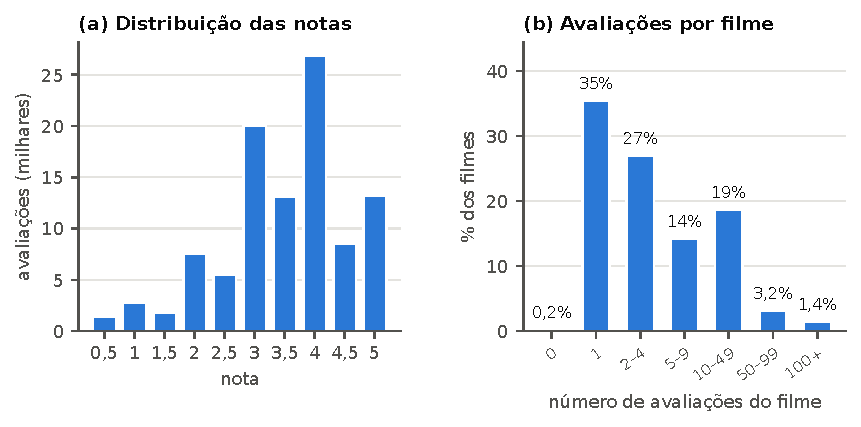
\includegraphics[width=0.92\textwidth]{figuras/fig_avaliacoes.pdf}
  \caption{Distribuição das notas (a) e do número de avaliações por filme (b).}
  \label{fig:avaliacoes}
\end{figure}

A preparação gerou dois produtos: um banco relacional e um índice vetorial.

\begin{enumerate}
  \item \textbf{Limpeza.} Título e ano separados (\code{Matrix, The (1999)} vira
        \enquote{The Matrix}, 1999); gêneros em uma tabela filme--gênero; tags normalizadas
        e agregadas por filme. Linhas com campos vazios foram removidas tabela a tabela
        (nenhuma no \emph{snapshot}): aplicada depois da junção, essa regra eliminaria os
        filmes sem tag, 84\% do acervo.
  \item \textbf{Média bayesiana.} Pela média simples, o topo eram filmes com uma ou duas
        notas 5 (296 filmes têm média 5,0). O banco guarda
        $\mathrm{WR} = \frac{v}{v+m}R + \frac{m}{v+m}C$, com $v$ avaliações do filme, média
        $R$, média global $C=3{,}50$ e $m=10$; o topo passa a ser \emph{Um Sonho de
        Liberdade}, \emph{O Poderoso Chefão} e \emph{Clube da Luta}. A mesma convenção vale
        no \emph{prompt} e no gabarito da avaliação.
  \item \textbf{Banco relacional.} SQLite com seis tabelas (filmes, gêneros, filme--gênero,
        tags, avaliações e metadados), descritas em \arq{docs/dicionario_dados.md}.
  \item \textbf{Índice vetorial.} Cada filme vira um texto com até 30 tags (ordenadas pelo
        número de usuários) e os gêneros em inglês e português. O título ficou de fora
        porque gerava falsos acertos (\enquote{comédia em família} trazia \emph{The Quiet
        Family}). O texto vira um vetor de 384 dimensões, e uma dimensão extra de
        popularidade faz o produto interno valer $0{,}9\cos(\mathbf{q},\mathbf{v}) +
        0{,}1\,p$, com $p=\ln(1+n)/\ln 330$ e $n$ avaliações; isso afasta filmes com uma ou
        duas notas. Os 9.742 vetores ficam no Firestore.
\end{enumerate}

% =============================================================================
\section{Modelagem e Análise dos Dados}
% =============================================================================

O \cg\ é um grafo LangGraph (Figura~\ref{fig:grafo}) publicado na web, com o site no Firebase
Hosting e a API no Cloud Run, a cerca de US\$ 0,01 por pergunta.

\begin{figure}[!htbp]
\centering
\begin{tikzpicture}[
  font=\footnotesize,
  box/.style={draw=cinza!70, rounded corners=3pt, fill=white, align=left,
              inner sep=4pt, text width=#1, anchor=west},
  dark/.style={box=#1, fill=tinta, draw=tinta, text=white},
  route/.style={box=4.1cm, fill=fundo, draw=cinza!50},
  arr/.style={-{Stealth[length=2mm]}, thick, cinza},
  carr/.style={-{Stealth[length=2mm]}, thick, cinza, dashed}
]
\node[box=1.9cm] (q) at (0,0.4) {\textbf{Pergunta}\\+ 3 últimas\\trocas};
\node[dark=2.3cm] (cl) at (2.63,0.4) {\textbf{classify}\\o LLM monta\\o plano: rota,\\filtros e tema};
\node[route, fill=fundoazul, draw=azul!60] (sql) at (6.01,1.9) {\textbf{sql}: Text-to-SQL validado\\e executado no SQLite};
\node[route, fill=fundolaranja, draw=laranja!70] (vec) at (6.01,0.75) {\textbf{vector}: vizinhos mais\\próximos (banco vetorial)};
\node[route] (hyb) at (6.01,-0.4) {\textbf{hybrid}: busca vetorial\\ampla + filtros exatos};
\node[route, dashed] (out) at (6.01,-1.75) {\textbf{outro}: texto fixo, sem\\busca (fora do escopo)};
\node[dark=2.4cm] (ans) at (11.19,0.75) {\textbf{answer}\\o LLM escolhe\\IDs entre os\\candidatos e\\justifica};
\node[box=2.4cm] (resp) at (11.19,-1.75) {\textbf{Resposta}\\texto e cartões\\com dados\\do SQLite};
\draw[arr] (q) -- (cl);
\draw[carr] (cl.east) -- ++(0.3,0) |- (sql.west);
\draw[carr] (cl.east) -- ++(0.3,0) |- (vec.west);
\draw[carr] (cl.east) -- ++(0.3,0) |- (hyb.west);
\draw[carr] (cl.east) -- ++(0.3,0) |- (out.west);
\draw[arr] (sql.east) -- ++(0.3,0) |- ([yshift=4.5mm]ans.west);
\draw[arr] (vec.east) -- (ans.west |- vec.east);
\draw[arr] (hyb.east) -- ++(0.3,0) |- ([yshift=-4.5mm]ans.west);
\draw[arr] (ans) -- (resp);
\draw[arr] (out) -- (resp);
\end{tikzpicture}
\caption{Grafo do \cg. Setas tracejadas: aresta condicional decidida pela rota do plano.}
\label{fig:grafo}
\end{figure}

\begin{itemize}
  \item \textbf{classify}: o LLM transforma a pergunta em um plano estruturado com a rota, os
        filtros (gêneros, anos, nota) e o tema reescrito em inglês no vocabulário das tags.
        A reescrita foi decisiva: \enquote{melancólico sobre memória} passou a trazer
        \emph{Memento} e \emph{Brilho Eterno} em vez de \emph{Regarding Henry}.
  \item \textbf{sql}: o LLM escreve a consulta, e um validador só aceita um único
        \code{SELECT} nas tabelas do acervo, com até 50 linhas. O banco executa só para
        leitura, e um erro volta ao modelo uma vez.
  \item \textbf{vector} e \textbf{hybrid}: o tema vira vetor e o Firestore devolve os
        vizinhos mais próximos (60 no \code{vector}). Um filme citado (\enquote{algo como
        Matrix}) soma seu vetor à busca e sai da lista. O \code{hybrid} busca 200 vizinhos e
        aplica os filtros do plano em SQL parametrizado.
  \item \textbf{answer}: o LLM escolhe identificadores entre até 15 candidatos e justifica
        cada um. Título, ano, gêneros e nota exibidos vêm do banco, e um identificador fora
        dos candidatos é descartado. A garantia contra dados inventados é da arquitetura,
        não do \emph{prompt}.
\end{itemize}

\textbf{Avaliação.} Escrevemos 95 perguntas com gabarito: 30 objetivas, com SQL de
referência; 30 semânticas e 30 mistas, com relevância de cada filme dada por um juiz LLM
(0, 1 ou 2) e, nas mistas, restrições conferidas no banco; e 5 fora do escopo. Cada pergunta
rodou em cinco configurações: o \cg\ roteado; só SQL, só vetorial e só híbrido (mesmo plano,
muda só a busca); e só LLM, cujas afirmações foram conferidas no MovieLens (o título existe?
ano $\pm1$, gêneros e nota $\pm0{,}3$ corretos?). As métricas foram acerto exato
(objetivas), precisão@5 (semânticas), fração de filmes relevantes e dentro dos filtros entre
os 5 primeiros (mistas) e taxa de itens com dado fabricado. As comparações são pareadas por
pergunta, com $\alpha=5\%$ e correção de Holm \cite{holm1979}: McNemar exato para H1
\cite{mcnemar1947}, Wilcoxon para H2 e H3 \cite{wilcoxon1945} e Fisher para H4
\cite{fisher1922}.

% =============================================================================
\section{Apresentação e discussão dos resultados}
% =============================================================================

\textbf{Roteamento.} O \code{classify} acertou a rota de 93 das 95 perguntas (97,9\%). Os
dois erros foram pedidos semânticos com gênero implícito (\enquote{filme leve para ver com a
família} e \enquote{guerra crua e realista}) enviados ao modo híbrido, onde tiveram
precisão@5 de 80\% e 100\%.

\begin{table}[!htbp]
\centering
\caption{Testes das hipóteses (30 perguntas por categoria; p ajustado por Holm).}
\label{tab:hipoteses}
\small
\begin{tabularx}{\textwidth}{@{}l>{\raggedright\arraybackslash}p{3.0cm}>{\raggedright\arraybackslash}X>{\raggedright\arraybackslash}p{3.3cm}l@{}}
\toprule
 & \textbf{Métrica} & \textbf{Resultado} & \textbf{Teste} & \textbf{Veredito} \\
\midrule
H1 & acerto exato (objetivas) & SQL 100\%; vetorial 17\%; híbrido 17\% & McNemar,~$p<0{,}001$ & confirmada \\
H2 & precisão@5 (semânticas) & vetorial 91\%; SQL 80\% & Wilcoxon, $p=0{,}058$ & não confirmada \\
H3 & relevantes e nos filtros@5 (mistas) & híbrido 87\%; SQL 54\%; vetorial 41\% & Wilcoxon, $p<0{,}001$ & confirmada \\
H4 & itens com dado fabricado & roteado 0\% (0/373); só LLM 17,1\% (87/508) & Fisher, $p<0{,}001$ & confirmada \\
\bottomrule
\end{tabularx}
\end{table}

\begin{figure}[!htbp]
  \centering
  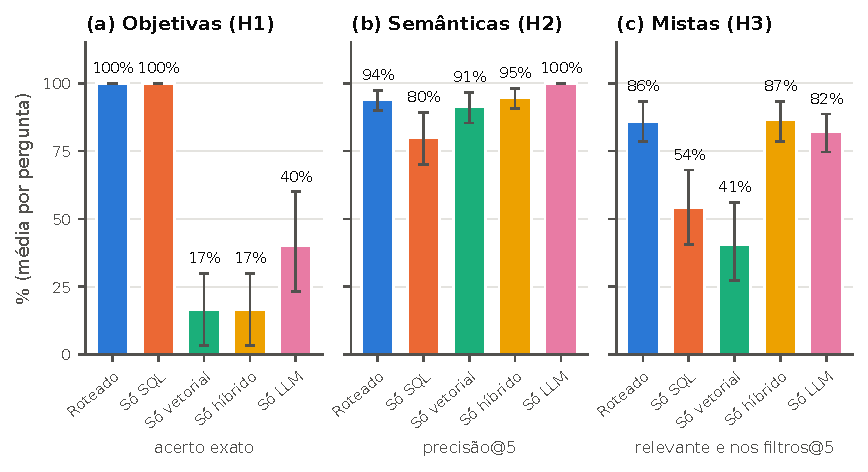
\includegraphics[width=0.92\textwidth]{figuras/fig_hipoteses.pdf}
  \caption{Métricas de H1 a H3 por configuração, com intervalos de confiança de 95\%
  (\emph{bootstrap} sobre as perguntas).}
  \label{fig:hipoteses}
\end{figure}

\textbf{Hipóteses} (Tabela~\ref{tab:hipoteses} e Figura~\ref{fig:hipoteses}). Em H1, o SQL
acertou as 30 perguntas objetivas; as buscas vetorial e híbrida acertaram só 5, todas de
valor único (como a nota de um filme citado), e nenhum \emph{ranking}. Em H2, a busca
vetorial ficou 11 pontos à frente do SQL, mas sem significância: com 30 perguntas o teste
tem pouco poder, e o SQL forçado não foi um adversário fraco, porque em 25 das 30 perguntas
procurou palavras do tema nas tags. Em H3, os mecanismos falham de forma complementar: o
vetorial acerta o tema e ignora ano e nota; o SQL respeita os filtros, mas não representa
\enquote{leve} ou \enquote{filosófico}. Em H4, 87 dos 508 itens do chatbot só com LLM
tinham dado errado (53 com gênero que o filme não tem, 47 com nota errada), e 43 das 90
respostas tinham ao menos um erro; no \cg, foram zero em 373 itens.

\textbf{Discussão.} O sistema roteado empatou com o melhor mecanismo de cada categoria
(diferenças de até 0,7 ponto, $p\ge0{,}32$), ou seja, o roteador obtém o desempenho de quem
escolhesse manualmente o mecanismo certo. O chatbot só com LLM teve a maior relevância
segundo o juiz (100\% nas semânticas), mas o juiz é o mesmo modelo e tende a aprovar filmes
famosos, e essa relevância veio acompanhada de dados errados que o usuário não tem como
identificar. O \cg\ respondeu em 5,3 s na mediana, a US\$ 0,009 por pergunta. As principais
limitações são o tamanho da amostra (30 perguntas por categoria), o uso de parte das
perguntas durante o desenvolvimento e o juiz automático, que precisaria de revisão humana
por amostragem.

% =============================================================================
\section{Conclusões}
% =============================================================================

Combinar consultas estruturadas e busca semântica com roteamento funcionou: cada mecanismo é
o melhor no seu tipo de pergunta (H1 e H3 confirmadas, H2 com tendência favorável), o
roteador acerta 97,9\% das rotas e o sistema empata com o melhor mecanismo em cada
categoria. O resultado mais forte é H4: nenhum dado errado chegou ao usuário, contra 17,1\%
dos itens no chatbot só com LLM, porque o modelo apenas escolhe entre candidatos e todo dado
exibido vem do banco. A preparação dos dados (média bayesiana, perfis sem título,
popularidade no vetor) pesou tanto quanto o modelo. Como próximos passos, propomos mais
perguntas semânticas para testar H2 com poder suficiente, um conjunto de teste novo,
revisão humana do juiz e sinopses do TMDb para os 84\% de filmes sem tag.

\bibliography{referencias}

\end{document}
